%\documentclass{slides}
\documentclass{beamer}
\usepackage[utf8]{inputenc}
%\usepackage{portland}
\usepackage{graphicx}
%\usepackage{pdflscape}

%========Hierboven niets veranderen!========%

\usepackage[export]{adjustbox}% for the second solution
\usepackage{amsmath}
\usepackage{amsfonts}
\usepackage{amssymb}
\usepackage{mathtools}
\usepackage{scalerel}
\usepackage[normalem]{ulem}
\usepackage{wisjab}

\setlength\fboxsep{4mm}
\setlength\fboxrule{0.8mm}

\definecolor{mygreen}{rgb}{0, 0.5, 0}
\def\gemph#1{{\color{mygreen}#1}}
\def\ck{\cellcolor{green!05}}

\def\lbt{\small QC$^2$ meeting 02-10-2023} %Titel die linksboven verschijnt
\parindent=0pt
%\makesavenoteenv{tabular}
\renewcommand{\thefootnote}{\arabic{footnote}}

\DeclareMathOperator{\tr}{tr}
\DeclareMathOperator{\sgn}{sgn}
\DeclareMathOperator{\poly}{poly}
\DeclareMathOperator{\Rea}{Re}
\DeclareMathOperator{\Ima}{Im}
\renewcommand{\Re}{\Rea}
\renewcommand{\Im}{\Ima}

\def\vc#1{\boldsymbol{\mathsf{#1}}}
\def\mt#1{\kern0.025em\mathsf{#1}\kern0.025em}
\def\mtg#1{\kern0.6pt\slantbox[-0.25]{$#1$}\kern-0.6pt}

\def\1{\mathds1}
\def\d{\mathsf d}
\def\e{\mathsf e}
\def\i{\mathsf i}
\def\lambdai{\lambda_{\sf i}}
\def\lambdaf{\lambda_{\sf f}}

\def\A{\mt A}
\def\H{\mt H}
\def\HCD{\mt H_{\sf CD}}
\def\U{\mt U}

\def\+{\kern0.0833em}
\def\:{\kern-0.07em}

\renewcommand{\thefootnote}{\arabic{footnote}}

\newenvironment{dia}[2]
{
	\begin{frame}
	\vspace{1mm}
	{\small #1}
	\hfill
    {\small\bf\textcolor{blue}{#2}}
	\vspace{3mm}
	\hrule
	\bigskip
}
{
	\vfill
	\end{frame}
}

\frenchspacing

\begin{document}
%\landscape

\begin{dia}{\lbt}{}
\vspace*{0.5cm}
\begin{center}
\begin{large}
QC$^2$ meeting 02-10-2023 \\[1.25cm]
\end{large}
\begin{LARGE}
\textcolor{mygreen}{Digitised counterdiabatic driving with $\Delta^{-?}$ gap scaling}\\[1.25cm]
\end{LARGE}
Dyon van Vreumingen
\end{center}
\end{dia}

\begin{dia}{\lbt}{Contents}
$ $\\
\begin{itemize}
    \setlength{\itemsep}{3mm}
    \item Adiabatic state preparation and counterdiabatic driving \pause
    \item Digitised CD
\end{itemize}
\vspace{3cm}
\end{dia}

\begin{dia}{\lbt}{}
\vspace{2.5cm}
\begin{center}
\begin{LARGE}
\textcolor{mygreen}{Adiabatic state preparation and counterdiabatic driving}
\end{LARGE}
\end{center}
\vspace*{1.5cm}
\end{dia}

\begin{dia}{\lbt}{Adiabatic state preparation}
Given: \pause
\begin{itemize}
    \item family of continuously parametrised hamiltonians $\H(\lambda)$ \pause
    \item system prepared in eigenstate $\ket{n(\lambdai)}$ of $\H(\lambdai)$ for some $\lambdai$ \pause
\end{itemize}
$ $\\[-2mm]
Objective: find corresponding eigenstate (ground state) of $\H(\lambdaf)$ for some $\lambdaf$ \pause \\[4mm]
Example: $\H(\lambda) = \mt h + \lambda \mt V$, $\lambdai = 0$, $\lambdaf = 1$ \pause \\[4mm]
\gemph{Adiabatic theorem}: \pause
\begin{itemize}
    \item slowly (and continuously) vary $\lambda$ with time, such that $\lambda(t=0) = \lambdai$ and $\lambda(t=T) = \lambdaf$ \pause
    \item time-evolved state w.r.t. time-dependent hamiltonian $\H(\lambda(t))$ approximates $\ket{n(\lambdaf)}$
\end{itemize}
\vspace{-1cm}
\end{dia}

\begin{dia}{\lbt}{Adiabatic state preparation}
\begin{center}
    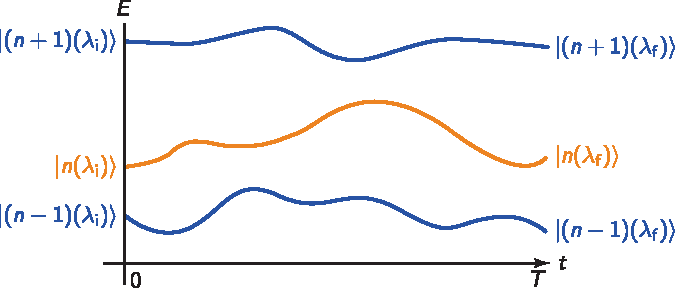
\includegraphics[width=\textwidth]{fig/adiabatisch_a.pdf}
\end{center}
$ $ \\[-4mm]
{\color{white}
More precisely: an adiabatic sweep of duration $T \geq O(\epsilon^{-1/2 }\Delta_{\sf min}^{-3})$
will produce a state with fidelity $\geq 1 - \epsilon$
}
\vspace{-1cm}
\end{dia}

\begin{dia}{\lbt}{Adiabatic state preparation}
\begin{center}
    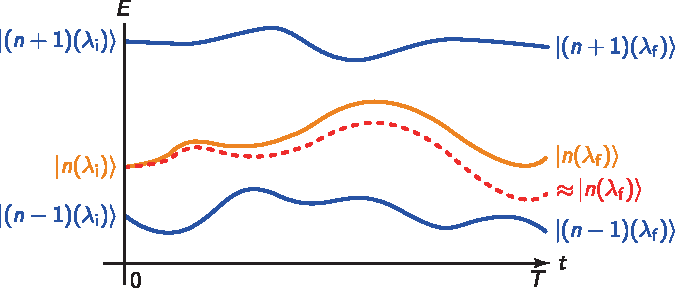
\includegraphics[width=\textwidth]{fig/adiabatisch_b.pdf}
\end{center}
$ $ \\[-4mm]
{\color{white}
More precisely: an adiabatic sweep of duration $T \geq O(\epsilon^{-1/2 }\Delta_{\sf min}^{-3})$
will produce a state with fidelity $\geq 1 - \epsilon$
}
\vspace{-1cm}
\end{dia}

\begin{dia}{\lbt}{Adiabatic state preparation}
\begin{center}
    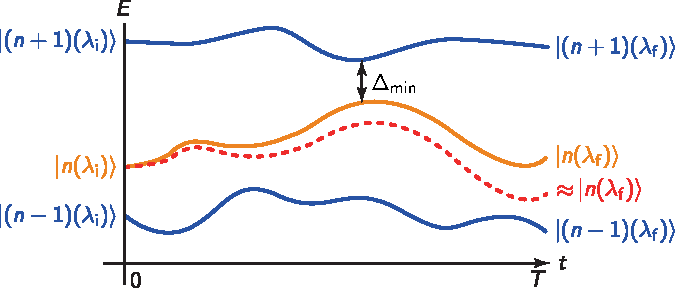
\includegraphics[width=\textwidth]{fig/adiabatisch_c.pdf}
\end{center}
$ $ \pause \\[-4mm]
More precisely: an adiabatic sweep of duration $T \geq O(\epsilon^{-1/2 }\Delta_{\sf min}^{-3})$
will produce a state with fidelity $\geq 1 - \epsilon$
\vspace{-1cm}
\end{dia}

\begin{dia}{\lbt}{Counterdiabatic driving}
Lack of fidelity caused by \gemph{nonadiabatic transitions} into other eigenstates \pause \\[4mm]
Idea: time-evolve with $\HCD(t) = \H(t) + \text{something}(t)$ such that transitions are suppressed and we can evolve faster \pause \\[6mm]
\begin{center}
    \begin{tabular}{ccc}
        adiabatic & non-adiabatic & counter-diabatic \\[2mm]
        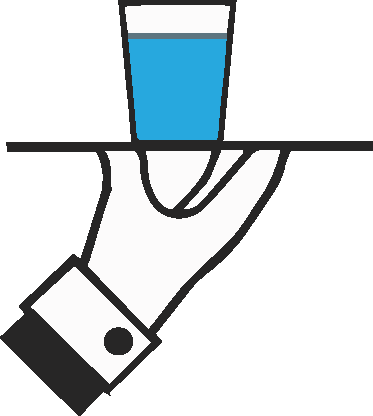
\includegraphics[scale=0.4]{fig/ober_a.pdf} &
        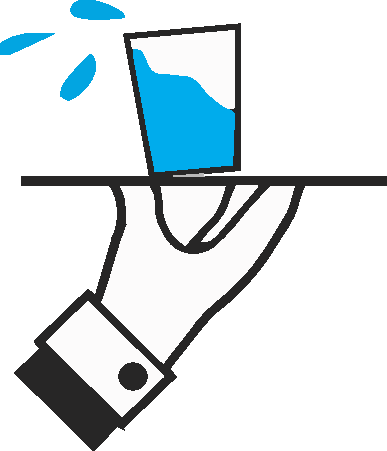
\includegraphics[scale=0.4]{fig/ober_b.pdf} &
        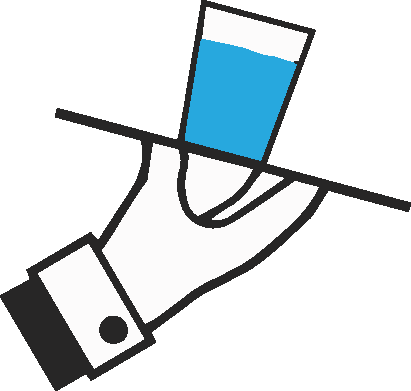
\includegraphics[scale=0.4]{fig/ober_c.pdf}
    \end{tabular}
\end{center}
\vspace{-1cm}
\end{dia}

\begin{dia}{\lbt}{Counterdiabatic driving}
Time-dependent Schr\"odinger equation:
\begin{align*}
    \i \+ \d_t \ket{n(\lambda(t))} = \H(\lambda(t)) \ket{n(\lambda(t))}
\end{align*} \pause
Define $\U(\lambda)$ such that $\U(\lambda) \ket{n(\lambdai)} = \ket{n(\lambda)}$ \pause \\[4mm]
Change to rotating frame that moves with eigenstates:
\begin{align*}
    \i \+ \d_t \ket{n} = [\mt U\t \mt H \mt U {\color{red} {} - \i \+ \dot\lambda \+ \mt U\t \partial_\lambda \mt U}] \ket{n}
\end{align*}
$ $ \pause \\[-2mm]
If we instead evolve with $\U\t\HCD\U := \U\t\H\U {\color{red} {} + \i \+ \dot\lambda \+ \mt U\t \partial_\lambda \mt U}$, then $\ket n$ remains \gemph{stationary} in rotating frame \pause \\[4mm]
In lab frame, $\HCD := \H + \i \+ \dot\lambda \+ \partial_\lambda \mt U \mt U\t$ suppresses all transitions
\vspace{-1cm}
\end{dia}

\begin{dia}{\lbt}{Counterdiabatic driving}
Operator $\A := \i \+ \partial_\lambda \mt U \mt U\t$ is known as \gemph{adiabatic gauge potential} \pause \\[4mm]
It is simply the derivative operator $\i \+ \partial_\lambda$:
\begin{align*}
    \bra{m(\lambda)} \mt A \ket{n(\lambda)} &= \i \+ \bra{m(\lambda)} \partial_\lambda \mt U \ket{n(\lambdai)} \\
    &= \i \+ \bra{m(\lambda)} \partial_\lambda \ket{n(\lambda)}
\end{align*} \pause
If we know $\A(\lambda)$, we can perform \gemph{transitionless} driving for \gemph{any driving time T} (i.e. also in limit $T\to0$)! \pause \\[4mm]
However, two issues: \pause
\begin{itemize}
    \item we can only compute $\mt A(\lambda)$ at finite number of points \pause
    \item computing $\mt A(\lambda)$ is generally exponentially hard :(
\end{itemize}
\vspace{-1cm}
\end{dia}

\begin{dia}{\lbt}{Counterdiabatic driving}
Heuristic to approximate AGP: \pause
\begin{itemize}
    \item define parametrised operator ansatz $\mt X(\vcg\alpha)$ \pause
    \item minimise action function
    \begin{align*}
        S(\mt X) := \tr[\mt G(\mt X)^2], \quad \mt G(\mt X) := \partial_\lambda \H + \i \+[\mt X, \mt H]
    \end{align*} 
    \item provably, if $S = 0$, then $\mt X = \mt A$ \pause
\end{itemize}
$ $\\[-2mm]
General ansatz: nested commutator ansatz
\begin{align*}
    \mt A^{(\ell)} = \i \sum_{k=1}^{\ell} \alpha_k \underbrace{[\mt H, [\mt H, \ldots[\mt H}_{2k-1}, \partial_\lambda \mt H]]]
\end{align*} \pause
Provably, if $\ell\to\infty$, then $\exists \+ \alpha_1, \ldots, \alpha_\ell$ s.t. $\mt A^{(\ell)} = \mt A$
\vspace{-1cm}
\end{dia}

\begin{dia}{\lbt}{}
\vspace{2.5cm}
\begin{center}
\begin{LARGE}
\textcolor{mygreen}{Digitised counterdiabatic driving}
\end{LARGE}
\end{center}
\vspace*{1.5cm}
\end{dia}

\begin{dia}{\lbt}{Digitised CD}
Goal: \pause
\begin{itemize}
    \item implement approximate CD directly on (gate-based) QC, avoiding heuristics \pause
    \item improve scaling as compared to bare adiabatic driving \pause
    \begin{itemize}
        \item recall: driving time $T \geq O(\epsilon^{-1/2}\Delta_{\min}^{-3})$ for fidelity $1 - \epsilon$ \pause
    \end{itemize}
\end{itemize}
$ $\\[-2mm]
We want to approximate the unitary
\begin{align*}
    \mt U(\lambdai, \lambdaf) = \sum_n \ket{n(\lambdaf)}\bra{n(\lambdai)} = \mathcal P \exp \bigg[ \! -\!\i \int_0^T \d t \, (\mt H(t) + \dot\lambda \+ \mt A(t)) \bigg]
\end{align*}
{\color{white}
    First step: trotterise (or maybe something more clever? \@ Kareljan)
    \begin{align*}
        \mt U(\lambdai, \lambdaf) \approx \prod_k \exp[-\i \+ \delta\lambda \A(\lambda_k)]
    \end{align*}
}
\vspace{-1.4cm}
\end{dia}

\begin{dia}{\lbt}{Digitised CD}
Goal:
\begin{itemize}
    \item implement approximate CD directly on (gate-based) QC, avoiding heuristics
    \item improve scaling as compared to bare adiabatic driving
    \begin{itemize}
        \item recall: driving time $T \geq O(\epsilon^{-1/2}\Delta_{\min}^{-3})$ for fidelity $1 - \epsilon$
    \end{itemize}
\end{itemize}
$ $\\[-2mm]
We want to approximate the unitary
\begin{align*}
    \mt U(\lambdai, \lambdaf) = \sum_n \ket{n(\lambdaf)}\bra{n(\lambdai)} = \mathcal P \exp \bigg[ \! -\!\i \int_{\lambdai}^{\lambdaf} \d\lambda \+ \mt A(\lambda) \bigg]
\end{align*} \pause
First step: trotterise (or maybe something more clever? @Kareljan)
\begin{align*}
    \mt U(\lambdai, \lambdaf) \approx \prod_k \exp[-\i \, \delta\lambda \, \A(\lambda_k)]
\end{align*}
\vspace{-1.4cm}
\end{dia}

\begin{dia}{\lbt}{Digitised CD}
To implement $\exp[-\i \, \delta\lambda \, \A(\lambda)]$, we make use of two facts: \pause
\begin{itemize}
    \item by the Hellman-Feynman theorem,
    \begin{align*}
        \bra m \A \ket n = \frac{\bra m \partial_\lambda\H \ket n}{\i \+ \omega_{mn}} \quad \text{where } \omega_{mn} = E_m - E_n
    \end{align*}
    \item function $\hat f(\omega) = 1/\i\omega$ is the Fourier transform of $\frac12 \sgn(\tau)$ \pause
\end{itemize} 
$ $\\[-4mm]
Therefore
\begin{align*}
    \A = \frac12 \int_{-\infty}^\infty \d\tau \, \sgn(\tau) \, \e^{-\i\H\tau} \partial_\lambda \H \+ \e^{\i\H\tau} \\[-8mm]
\end{align*} \pause
since
\begin{align*}
    \bra m \A \ket n = \frac12 \int_{-\infty}^\infty \d\tau \, \sgn(\tau) \, \e^{-\i(E_m - E_n)\tau} \bra m \partial_\lambda \H \ket n
\end{align*}
\vspace{-1.4cm}
\end{dia}

\begin{dia}{\lbt}{Digitised CD}
Idea: \pause
\begin{itemize}
    \item cut off integral at finite value $a$ \pause
    \item approximate with Riemann sum and Trotter product \pause
\end{itemize}
\begin{align*}
    \mt A &\approx \frac12 \int_{-a}^a \d\tau \, \sgn(\tau) \, \e^{-\i\H\tau} \partial_\lambda \H \+ \e^{\i\H\tau} \\[1mm]
    &\approx \frac12 \sum_{\tau_\kappa=-a}^{\tau_\kappa=a} \delta\tau \, \sgn(\tau_\kappa) \, \e^{-\i\H\tau_\kappa} \partial_\lambda \H \+ \e^{\i\H\tau_\kappa} \\[1mm]
    \e^{-\i \, \delta\lambda \, \A(\lambda)} &\approx \prod_{\tau_\kappa=-a}^{\tau_\kappa=a} \e^{-\i\H\tau_\kappa} \+ \e^{-\i \+ \delta\lambda \+ \delta\tau \sgn(\tau_\kappa) \+ \partial_\lambda \H/2} \, \e^{\i\H\tau_\kappa}
\end{align*} \pause
This approach uses $\displaystyle O\Big(\frac{a}{\delta\tau}\frac{|\lambdaf - \lambdai|}{\delta\lambda}\Big)$ operator exponentials
\vspace{-1cm}
\end{dia}

\begin{dia}{\lbt}{Digitised CD}
There's an issue with this cut-off method... \pause \\[4mm]
Cut off integral does not converge for $a\to\infty$:
\begin{align*}
    \frac12 \int_{-a}^a \d\tau \, \sgn(\tau) \, \e^{-\i\+\omega_{mn}\tau} = \frac{1 - \cos(a\+\omega_{mn})}{\i\+ \omega_{mn}}
\end{align*} \pause
Error uncontrollable since $\omega_{mn}$ are unknown \pause \\[4mm]
We add a \gemph{regulariser}:
\begin{align*}
    \frac12 \int_{-a}^a \d\tau \, \sgn(\tau) \, {\color{mygreen} \e^{-\omega_0^2\tau^2}} \+ \e^{-\i\+\omega_{mn}\tau} = \frac1{\i\+\omega_{mn}} + \frac1\i O(\e^{-\omega_0^2 a^2}) + \frac1\i O\Big(\frac{\omega_0^2}{\omega_{mn}^3}\Big)
\end{align*} \pause
Intuition: approximation accurate for $\omega_0 \ll |\omega_{mn}|$, $a \gg \omega_0^{-1}$
\vspace{-1cm}
\end{dia}

\begin{dia}{\lbt}{Error analysis}
We now have a number of errors from approximations \pause \\[4mm]
To achieve $1 - \text{fidelity} \leq O(\epsilon)$, each error term must be $\leq \epsilon$ \pause
\begin{center}
    \renewcommand{\arraystretch}{1.2}
    \begin{tabular}{c|c|c}
        error source & error & parameter choice \\ \hline
        regulariser & $O\big(\frac{\omega_0^2}{\Delta_{\sf min}^3}\big)$ & $\omega_0 \leq O(\epsilon^{1/2}\Delta_{\sf min}^{3/2})$ \pause \\
        integral cut-off & $O\big(\frac1{\omega_0^2 a} \e^{-\omega_0^2 a^2}\big)$ & $a \geq \tilde O(\epsilon^{-1/2}\Delta_{\min}^{-3/2})$ \pause \\
        Riemann sum & \sout{negligible} $\sim a^2 \+ \delta\tau^2$ & $\delta\tau^{-1} \geq \epsilon^{-1}\Delta_{\sf min}^{-3/2}$ \pause \\
        fixed $\lambda$ Trotter & ? & --- \\
        variable $\lambda$ Trotter & ? & $\delta\lambda^{-1} \geq {?}$ \pause
    \end{tabular}
\end{center}
We see $\displaystyle \frac a{\delta\tau}$ is already $\tilde O(\epsilon^{-3/2}\Delta_{\sf min}^{-3})$, so seemingly no gain here...
\vspace{-1cm}
\end{dia}

\begin{dia}{\lbt}{Open questions}
Is an improvement over $O(\epsilon^{-1/2}\Delta_{\sf min}^{-3})$ still within reach? \pause
\begin{itemize}
    \item How about the gate complexity of hamiltonian simulation for $\e^{\pm\i\H\tau_\kappa}$ and $\e^{-\i \+ \delta\lambda \+ \delta\tau \sgn(\tau_\kappa) \+ \e^{-\omega_0^2\tau^2} \partial_\lambda \H}$? \pause
    \begin{itemize}
        \item Typical results state $O(\poly(\delta\tau))$ complexity for implementing $\e^{-\i \mt O \delta\tau}$ (for some $\mt O$). Does this cancel out the $\delta\tau^{-1}$ in $\frac a{\delta\tau}$? \pause
    \end{itemize}
    \item Is there a better way to approximate
    \begin{align*}
        \exp\bigg[ \! -\!\i \, \delta\lambda \, \frac12 \int_{-a}^a \d\tau \, \sgn(\tau) \, \e^{-\omega_0^2\tau^2} \e^{-\i\H\tau} \partial_\lambda \H \+ \e^{\i\H\tau_\kappa} \bigg]
    \end{align*}
    than through a Riemann sum? \pause
    \item How does the error from variable $\lambda$ trotterisation scale? \pause
    \item Can we do better than Trotter methods?
\end{itemize}
\vspace{-1cm}
\end{dia}

\begin{dia}{\lbt}{}
\vspace{2.5cm}
\begin{center}
\begin{LARGE}
\textcolor{mygreen}{Questions?}
\end{LARGE}
\end{center}
\vspace*{1.5cm}
\end{dia}

\end{document}